\documentclass{beamer}

\usepackage[T1]{fontenc}
\usepackage{inputenc}

\usepackage{amsmath}
\usepackage{listings}
\lstset{
  basicstyle=\footnotesize,
  language=Caml,
  showstringspaces=false,
}


\usetheme{Boadilla}
\usecolortheme{dolphin}
\useoutertheme{infolines}


\setbeamertemplate{footline}
{
  \leavevmode%
  \hbox{%
  \begin{beamercolorbox}[wd=.333333\paperwidth,ht=2.25ex,dp=1ex,center]{author in head/foot}%
    \usebeamerfont{author in head/foot}\insertshortauthor%~~\beamer@ifempty{\insertshortinstitute}{}{(\insertshortinstitute)}
  \end{beamercolorbox}%
  \begin{beamercolorbox}[wd=.333333\paperwidth,ht=2.25ex,dp=1ex,center]{title in head/foot}%
    \usebeamerfont{title in head/foot}\insertshorttitle
  \end{beamercolorbox}%
  \begin{beamercolorbox}[wd=.333333\paperwidth,ht=2.25ex,dp=1ex,right]{date in head/foot}%
    \usebeamerfont{date in head/foot}\insertshortdate{}\hspace*{2em}
    \insertframenumber{} / \inserttotalframenumber\hspace*{2ex}
  \end{beamercolorbox}}%
  \vskip0pt%
}

\title{Filtering properties}
\author[Maxime Puys]{Maxime Puys\\~\\Supervision: Marie-Laure Potet \and Jean-Louis Roch}
\date{2015-02-26}

\graphicspath{{assets/}}

\begin{document}

\begin{frame}
    \maketitle
\end{frame}

\begin{frame}
    \frametitle{Debriefing on 2015-02-13 1/2}

    In the slides:
    \begin{itemize}
        \item A general overview of possible security issues and answers at several levels:
            \begin{itemize}
                \item Availability
                \item Integrity
                \item Confidentiality
                \item Authentication
                \item Freshness, replay attacks
                \item Traceability
                \item Maintenance
            \end{itemize}
            \vfill
        \item Not limited to the problematic of ARAMIS.
            \vfill
        \item A quick state of the art on technologies.
            \vfill
        \item A more in depth explanation on the contents of ANSSI documents.
    \end{itemize}
\end{frame}

\begin{frame}
    \frametitle{Debriefing on 2015-02-13 2/2}
    
    Discussions:
    \begin{itemize}
        \item Integrity of the module itself.
            \vfill
        \item Being able to recognize a true module on the network.
            \vfill
        \item Strong authentication.
            \vfill
        \item ISA 624463.
            \vfill
        \item Replay attacks.
            \vfill
        \item Passwords made accessible to the module.
    \end{itemize}
\end{frame}

\begin{frame}
    \frametitle{No global view}

    \begin{block}{Temporally}
        A process requires several commands, possibly bidirectional (request/answers).\\
        \medskip
        We do not have a global view of the whole process but only the command exchanged before and at a certain time $t$.
    \end{block}
    \vfill
    \begin{block}{Spatially}
        Let's say A and B exchange messages M : A <---M---> B\\
        We have no idea of the local state of A and B.
    \end{block}
\end{frame}

\begin{frame}
    \frametitle{Architecture}

    \begin{figure}[htb]
        \centering
        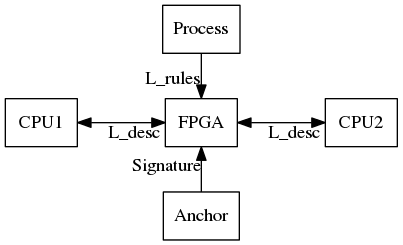
\includegraphics[scale=.35]{archi}
    \end{figure}
    \vfill
    L\_desc = Description language for applicative data.\\
    \medskip
    L\_rules = Description language for rules.
\end{frame}

\begin{frame}
    \frametitle{L\_desc}

    Textual subset of commands:
    \vfill
    \begin{itemize}
        \item[~] L\_desc ::=
        \begin{itemize}
            \item[~] modbus modbusCommand |
            \item[~] ftp ftpCommand
        \end{itemize}
        \item[~] modbusCommand ::= 
        \begin{itemize}
            \item[~] read reg |
            \item[~] write reg value
        \end{itemize}
        \item[~] ftpCommand ::=
        \begin{itemize}
            \item[~] get filename |
            \item[~] put filename filename |
            \item[~] ...
        \end{itemize}
    \end{itemize}
    \vfill
    $\Rightarrow$ [LIV01] Already puts a restriction on commands (and authorized applications).
\end{frame}

\begin{frame}
    \frametitle{L\_rules}

    Different possibilities to specify L\_rules follow.
\end{frame}

\begin{frame}
    \frametitle{On an example}

    \begin{figure}[htb]
        \centering
        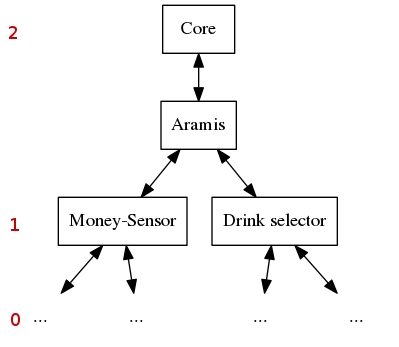
\includegraphics[scale=.3]{example}
    \end{figure}
    \vfill
    \begin{block}{Money-Sensor}
        var {\bf Paid}: Set to {\em 1} when paid. (Assume, everything has the same price).\\
        var {\bf CashOut}: If set to {\em 1}, then release the change.
    \end{block}
    \vfill
    \begin{block}{Drink selector}
        var {\bf Selected}: Set to {\em 1} when a drink is selected.\\
        var {\bf Deliver}: If set to {\em 1}, then delivers the drink.
    \end{block}
\end{frame}

\begin{frame}
    \frametitle{Normal behaviour}

    \begin{figure}[htb]
        \centering
        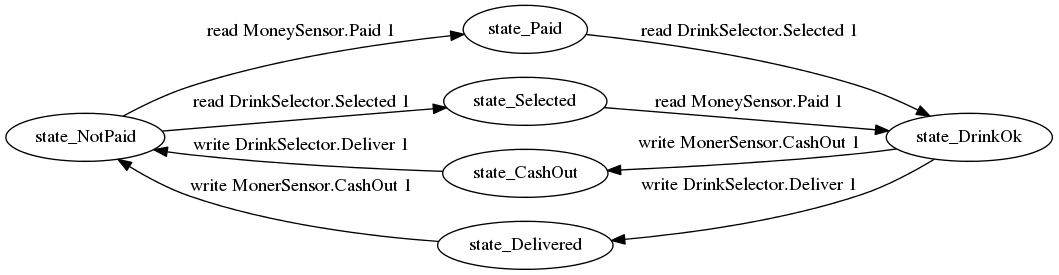
\includegraphics[scale=.32]{drink}
    \end{figure}
    \vfill
    Note: {\tt read MoneySensor.Paid 1} corresponds to the response/notification and not to the read request.
\end{frame}

\begin{frame}
    \frametitle{Regular expressions}

    \begin{block}{Shortening}
        Let:
        \begin{itemize}
            \item read MoneySensor.Paid 1 be {\bf Paid}
            \item write MoneySensor.CashOut 1 be {\bf CashOut}
            \item read DrinkSelector.Selected 1 be {\bf Selected}
            \item write DrinkSelector.Deliver.Paid 1 be {\bf Deliver}
        \end{itemize}
    \end{block}
    \vfill
    A regular expression verifying the normal behaviour could be:\\
    \medskip
    [(Paid.Selected + Selected.Paid)(Deliver.CashOut + CashOut.Deliver)]*
\end{frame}

\begin{frame}
    \frametitle{Temporal logic}

    \begin{itemize}
        \item[~] always(Paid before Deliver)
        \begin{itemize}
            \item[~] AND
        \end{itemize}
        \item[~] always(Paid before CashOut)
        \begin{itemize}
            \item[~] AND
        \end{itemize}
        \item[~] always(Selected before Deliver)
        \begin{itemize}
            \item[~] AND
        \end{itemize}
        \item[~] always(Selected before CashOut)
    \end{itemize}
    \vfill
    Transformed into automatas.\\
    {\em Difference  with regular expressions}: No one-to-one relation between events (similar with weak authentication).
\end{frame}

\begin{frame}
    \frametitle{Protocol verification}

    Generally offline with a global view of the system.
    \begin{itemize}
        \item[$\rightarrow$] Can not be used within ARAMIS.
    \end{itemize}
    \vfill
    \begin{block}{Inner working}
        witness(something) remembers seeing a message.\\
        request(something) if the requested message has not been witnessed earlier, an error is detected.
    \end{block}
    \vfill
    Can be used for example to check if a modbus response has been preceded by a request.
\end{frame}

\begin{frame}
    \frametitle{Blacklist of variable}

    \begin{itemize}
        \item[~] ReadOnly(MoneySensor.Paid);
        \item[~] WriteOnly(MoneySensor.CashOut);
        \item[~] ReadOnly(DrinkSelector.Selected);
        \item[~] WriteOnly(DrinkSelector.Deliver);
    \end{itemize}
    \vfill
    Writing on ReadOnly variable may directly affect the process!\\
    Reading WriteOnly variable gives nonsense values and can induce false interpretations.\\

    $\Rightarrow$ [LIV01] Also restricts which variable can be accessed in either way.
\end{frame}

\begin{frame}
    \frametitle{Interval constraints}

    Check if a data value is included in an interval or a set of authorized values.
    \vfill
    Example: $Temperature \in [500,1000]$\\
    \vfill
    Or: $Combustible \in \{Coal, Gas, Fuel\}$.
\end{frame}

\begin{frame}
    \frametitle{Stateful rules}
    
    Example:
    \vfill
    The filter accept a packet with SET\_TEMPERATURE 700, it remembers that $CurTemp = 700$.
    \vfill
    Then the filter sees another packet with SET\_TEMPERATURE n, it checks that $|n-CurTemp| < \delta$.
\end{frame}

\begin{frame}
    \frametitle{On file transfers}

    On file transfers, verification can apply on the file:
    \vfill
    \begin{itemize}
        \item Name (format, length, characters used, extension, ...)
            \vfill
        \item Size (not exceeding a certain limit)
            \vfill
        \item Type (maybe using the {\tt file} command)
            \vfill
        \item Contents (regular expressions on contents)
    \end{itemize}
\end{frame}

\begin{frame}
    \frametitle{OPC-UA}

    On OPC-UA objects, verification can apply on:
    \vfill
    \begin{itemize}
        \item Object format
              \begin{figure}[htb]
                  \centering
                  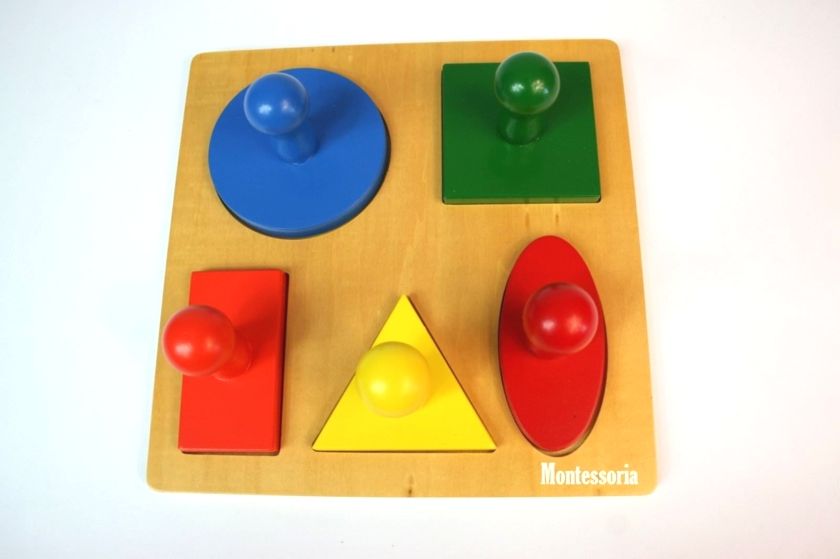
\includegraphics[scale=.15]{game}
              \end{figure}
            \vfill
        \item Contents (assertions on values)
    \end{itemize}
\end{frame}

\begin{frame}
    \frametitle{Conclusion}
    Several ways to filter an express properties (possibly mixed).
    \vfill
    Open question: Find a way to automatically specify L\_rules from a description of the process.
    \vfill
    \begin{center}
        Thanks for your attention!
    \end{center}
\end{frame}

\end{document}
